\documentclass{article}
\usepackage{amsmath} % equation, align, matrix, *, &, \\, \left, \right
\usepackage{graphicx} % figure
\usepackage{subcaption} % subfigure
\usepackage{comment} % To comment
\usepackage{hyperref} % To hyperlink and ref
\usepackage{enumitem} % To list
\usepackage[utf8]{inputenc}
\usepackage{wrapfig}
\usepackage{ulem}
\usepackage[backend=bibtex,style=numeric]{biblatex}
\usepackage{subfiles} %multifile latex projects
\usepackage{multirow}
\usepackage{booktabs}
\usepackage{placeins} %FloatBarrier

\graphicspath{{images/}{../images/}}

\bibliography{lib} 

\title{Idea de proyecto}
\author{Tim Reiprich \\ Tegshigzugder Otgonbayar \\ Maltagliati Luca}


\begin{document}
\maketitle
%\section{}
%\subsection{}
%\subsubsection{}

%\paragraph{}
%\subparagraph{}

\pagestyle{plain}
\pagenumbering{gobble} %hide page numbers

\paragraph*{Project: Height / capacity monitor}\mbox{}\\

\begin{comment}

Using an ultrasonic sensor or similar, monitor the height of a water tank, paper stack, garbage container, or similar. Think of multiple sensors to map the height in different positions of the container or different containers. To properly manage the filling / emptying of the container, monitoring the tank capacity, etc. Local warning by LEDs, minimum / maximum level alarms, etc.

The context and general description of the device to be designed
Basic scheme of system hardware (components and what information they exchange)
Summary of system operation
List of things you have to do to carry out the project, identifying what you know how to do and what you don't. 
Possible extensions

\end{comment}

\section{Context and general description of the device}

Our project focuses on the measurement of containers holding some kind of
liquid. Based on the volume of these containers alarms can be sent to the users
to notify them about the amount. To accomplish this, sensors will be used, that
can determine if the height of the volume is above or below a certain
threshold. \par

\subsection{Hardware scheme}

\begin{figure}
\label{scheme}
\hspace{-1cm}
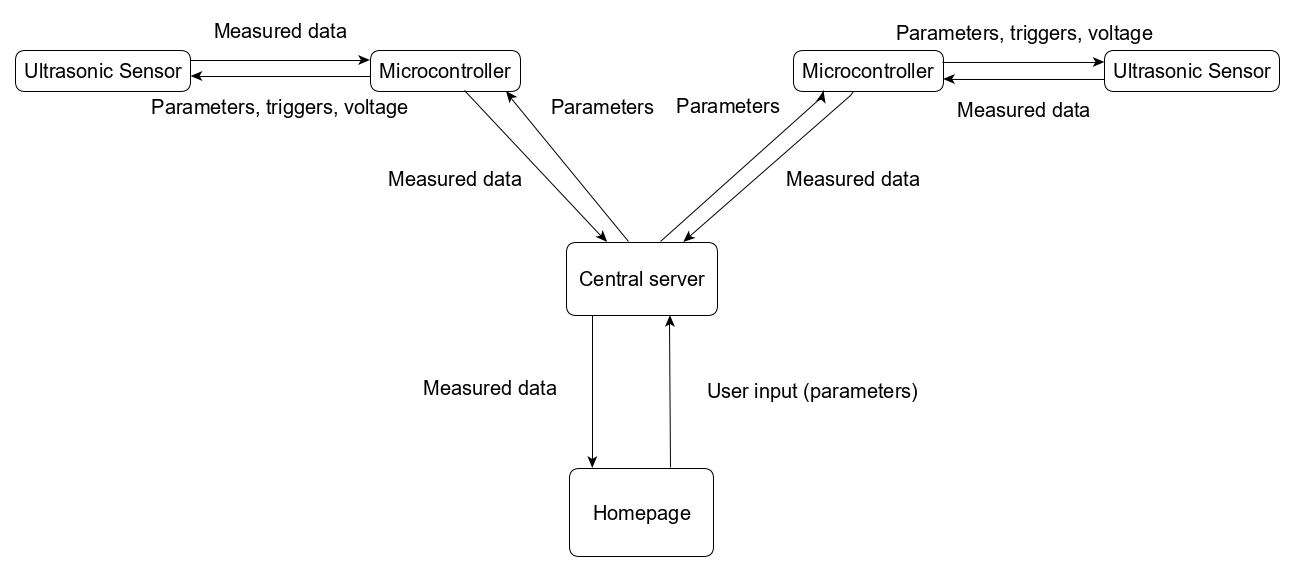
\includegraphics[scale=0.325]{images/circuit3.png}
\caption{Hardware scheme}
\end{figure}

The basic scheme of system hardware is described as follows: the main components
are the micro-controller as central server, the sensors and a web-page. The
sensors must be able to connect to the servers by a WiFi-connection and for this
we assume that the connection is robust and will be available in the given
environment. \par
\FloatBarrier
\subsection{Sensor}
We will use an ultrasonic sensor to measure the level of the liquid. An example of the sensor is \textit{Ultrasonic Sensor Module HC-SR-04 by Robokart}. 
We want to choose this approach because it is one of the best ways to sense proximity and detect levels with high reliability. Every sensor is connected to a microcontroller 
that collects the data and sends them to the central server via WiFi.  

Every container will have a microcontroller that is connected to at least one sensor (see figure \ref{sensorWithArduino}).
Certain specified heights of minimal and maximal volumes will be set, depending
on various factors, like the position of the container, the probability of it being used, 
the liquid type and as such.

\begin{figure}
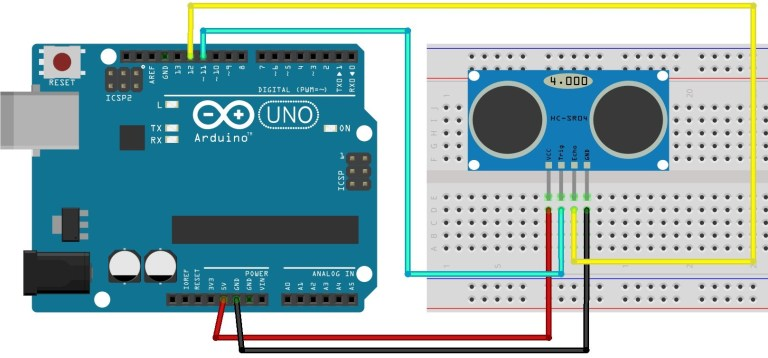
\includegraphics[scale=0.5]{sensorAndArduino.jpg}
\caption{Example of a sensor connected to a microcontroller}
\label{sensorWithArduino}
\end{figure}

\subsection{Central server}

We assume a LAN network to which the controllers and central
server are connected. Through this the microcontrollers will be able to communicate with the
central server by sending continuously the measurements of the liquid heights. 
The central server will perform checks on the thresholds and if needed send an alert to the user. 

As seen in Figure 1, the central server can also host a web page (e.g. with the Node-RED framework) in which the data are visualized in diagrams. 
This will be in an user-friendly interface, for it to be usable by non-technical people also.

\section{Steps of the project}

The first steps of the project will be to research about similar projects and
identifying platforms, programming languages and frameworks, choosing
the most suitable ones for our case.
Furthermore, the connection between devices
plays a crucial role, so we need to know what kind of protocols are needed.

Possible extensions are to also give specific numbers of the height of the
containers, how much volume they contain.
It is also possible to set up LEDs; their light will warn about specific
situations, e.g. when a container is empty a green light is shown, a red one when
is full.

\begin{comment}

\maketitle
\newpage

\pagenumbering{arabic} %show page numbers in arabic
\tableofcontents % from the section headings
\newpage

\listoffigures
 
\listoftables

%\listoftables
\newpage

\subfile{einleitung/einleitung}
\newpage

\subfile{grundlagen/grundlagen}
\newpage

\subfile{analyse/analyse}
\newpage

\printbibliography

\subfile{entwicklung/entwicklung}
\newpage

\subfile{evaluation/evaluation}
\newpage

\subfile{zusammenfassungundausblick/zusammenfassungundausblick}
\newpage

\end{comment}

\end{document}